\chapter{Experimental Results}
\label{chap:implementation}

\section{RSSI}
% Beacon RSS distributon ? \cite{barsocchi_detecting_2021} page 16.

Experiment results in \autoref{fig:beacon-dist-rssi} show that the distribution of RSSI is quite instable, as stated by the literature as one of the main challenges. The distributions are well spread over the values and don't follow a normal form.

\begin{figure}[h]
    \centering
    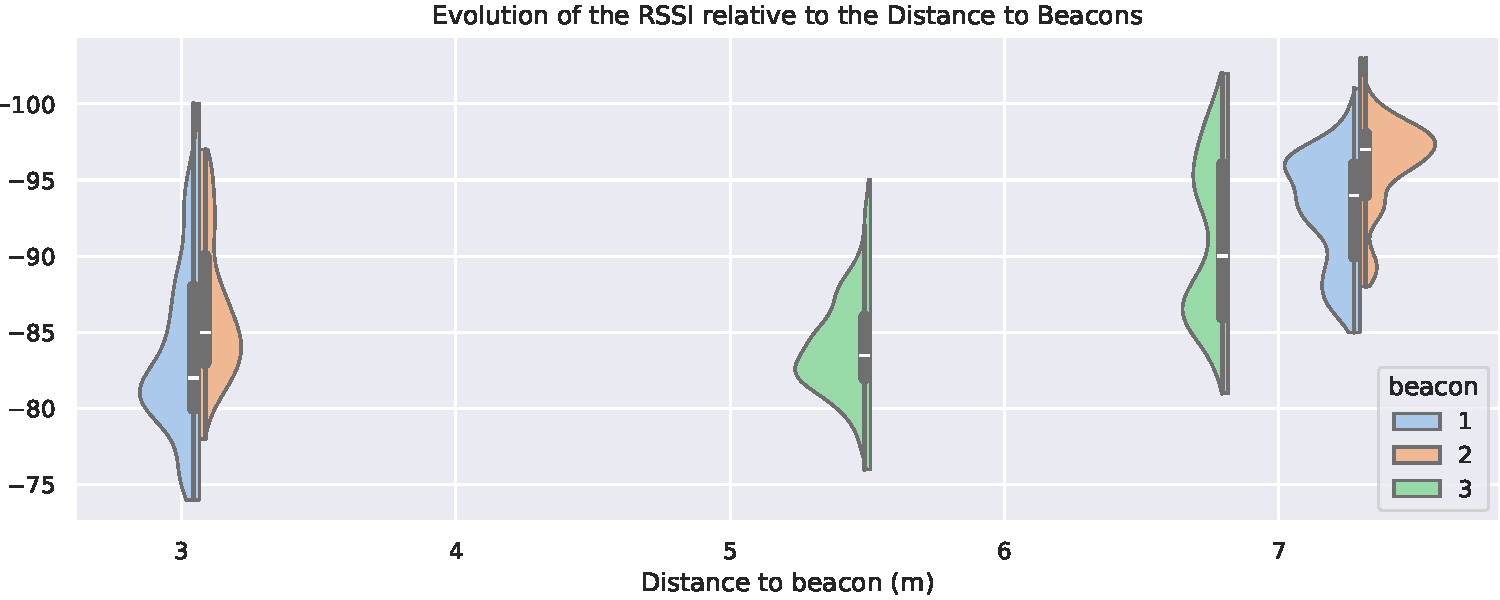
\includegraphics[width=\linewidth]{assets/beacon-dist-rssi.pdf}
    \caption{Variation in RSSI relative to Distance from Beacons}
    \label{fig:beacon-dist-rssi}
\end{figure}

\section{Distance to beacons}
% Relation between distance and precision ?

Experimental results of the variation of the raw distance error relative to the distance to beacons presented in \autoref{fig:beacon-dist-raw-error} confirms the findings of \cite{spachos_ble_2020}, where there is corelation between the error and the distance the beacons. Also, closer beacons leads to a smaller standard deviation.
 \autoref{fig:beacon-dist-filtered-error} shows that Kalman filtered distances reduce the standard deviation and improve precision when close to beacon and prevent extreme values when far the it. The differences between beacons are small when close to beacons, but increase with distance.

\begin{figure}[h]
    \centering
    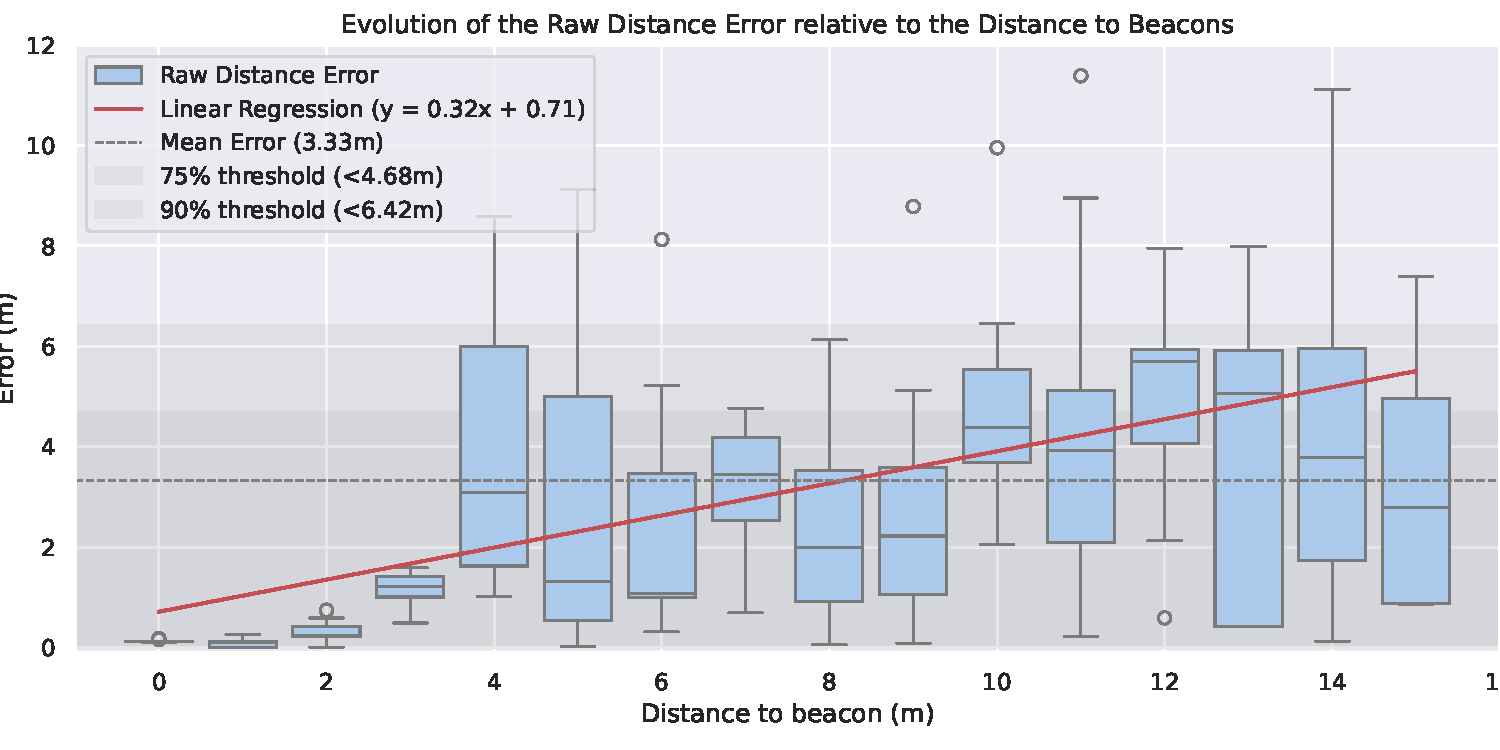
\includegraphics[width=\linewidth]{assets/beacon-dist-raw-error.pdf}
    \caption{Variation in Raw Distance Error relative to Distance from Beacons}
    \label{fig:beacon-dist-raw-error}
\end{figure}

\begin{figure}[h]
    \centering
    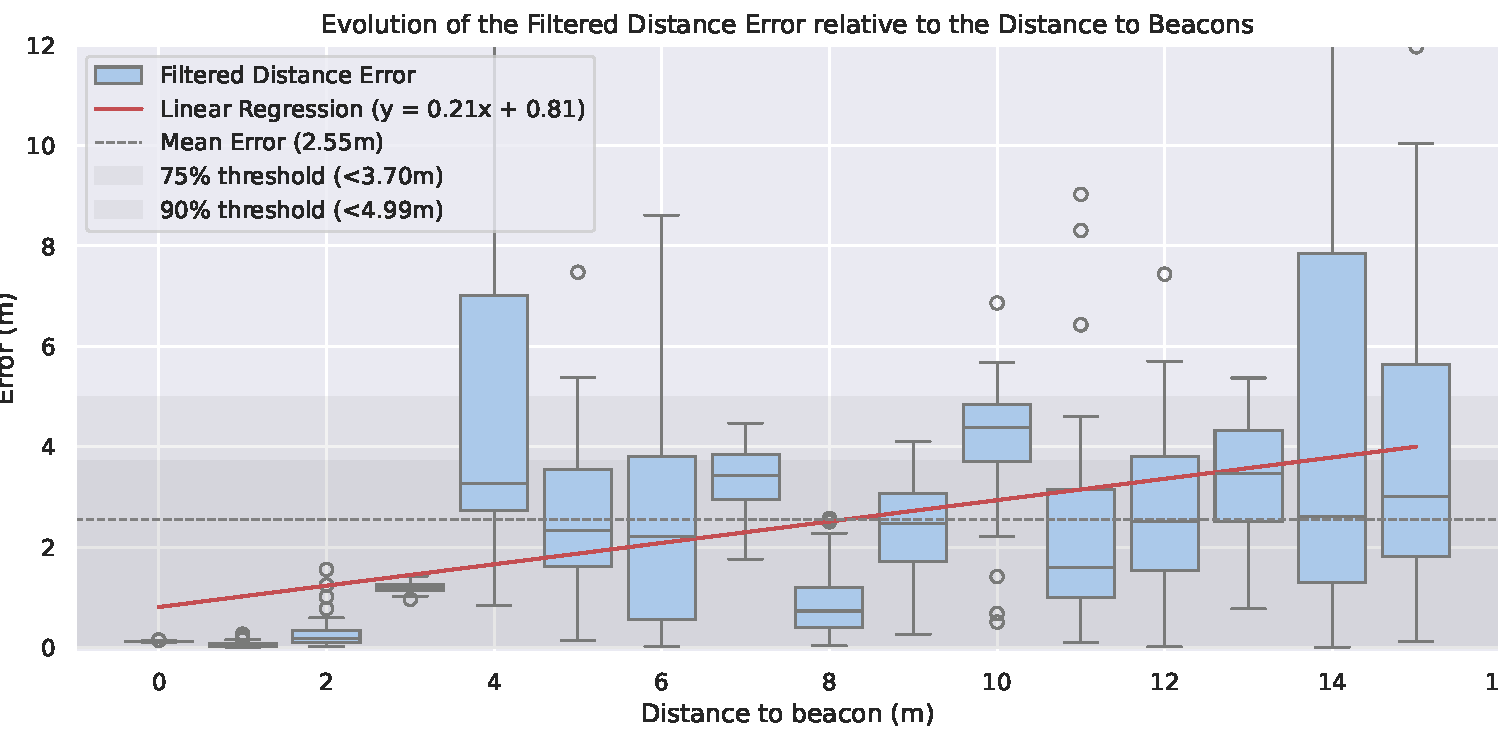
\includegraphics[width=\linewidth]{assets/beacon-dist-filtered-error.pdf}
    \caption{Variation in Filtered Distance Error relative to Distance from Beacons}
    \label{fig:beacon-dist-filtered-error}
\end{figure}



